\documentclass{report}
\usepackage[A4, top=2.5cm]{geometry}
\usepackage[utf8]{inputenc}
\usepackage{graphicx}
\usepackage{titlesec}
\usepackage{anyfontsize}
\usepackage{caption}
\usepackage{wrapfig}
\usepackage[export]{adjustbox}




\title{{DIGITAL IMAGE PROCESSING}\\{
} 
Assignement-1}


\author{ Gajendra singh rajput\\
19210076\\ 
Vasa vamsi krishna\\ 
19210112}
\date{September 2019}

\begin{document}

\maketitle
\tableofcontents
\newpage

   \section {Solution for Question No.2}

\noindent{The functions defined in the code are as followed:}\\

\noindent \textbf{1. Conncomp():}\\
 \textit{\noindent {\textbf{Input arguments}}}-Image(a), V intensity vector(in the form of array)(b), Connectivity(User defined).
\\*{\textit{\noindent{\textbf{Output argument-}}}} Connectivity, Image size, No. of connected components, PixelIDlist.\\
 
 \noindent \textbf{2. binarize ( ):}\\
\textit{\noindetnt{\textbf{Input arguments}}}- Image matrix(a), V intensity vector(in the form of array)(b). \\
\textit{\noindetnt{\textbf{{Output arguments}}}}- Binarized matrix(lab\_mat)(not given output).\\

\noindent \textbf{3. Level():}\\
\textit{\noindetnt{\textbf{Input argument}}}- Binarized matrix(lab\_mat), Image(a), V intensity vector (in the form of array)(b), connectivity, cur\_list[ ](to collect the labels in the first phase that are to be changed in next phase), conv\_list(to collect the labels the previously collected components are to be relabelled to).\\
\textit{\noindetnt{\textbf{Output argument}}}- Labeled matrix after phase-1(lab\_mat\_fin).\\

\noindent \textbf{4. Num\_order():}\\
\textit{\noindetnt{\textbf{Input arguments}}} - Labeled matrix after phase-2(lab\_mat\_fin).\\
\textit{\noindetnt{\textbf{Output arguments}}} - Labeled matrix numbering the components in chronological order(lab\_mat\_fin).\\

\noindent \textbf{5. PixelIDlist():}\\
\textit{\noindetnt{\textbf{Input arguments}}} - Labeled matrix after phase-2(lab\_mat\_fin), No. of the objects(Numobjects).\\
\textit{\noindetnt{\textbf{Output arguments}}} - The arrays of the positions index wise occupied by the particular mentioned components.\\

\noindent \textbf{6. member():}\\
\textit{\noindetnt{\textbf{Input arguments}}}- Any array(here b), Valued to be checked in the array(here a(row,col)). \\
\textit{\noindetnt{\textbf{Output arguments}}}- returns value of 'y' 1 if the value lies in array else 0.\\ 

\noindent \textbf{Explanation for the algorithm}:\\

\noindent This algorithm is coded using the basic inbuilt commands and only allowed inbuilt functions mentioned in the assignments. The functions called may not be reused again and again in this code, but can be used as a general function in upcoming projects.\\

\noindent \textbf{Step-1:} Binarizing the given image using V intensity vector.\\

\noindent The pixels in the image matrix are re-assigned new values as follows:
\begin{itemize}
\item If the intensity value of the pixel lies in the V intensity vector, the element will be re-assigned as 1.
\item If the value does not lie in the vector V, it will be re-assigned as 0. The finally  established matrix is given as input to the phase-1 of the sequential algorithm.\\
\end{itemize}

\noindent \textbf{Step-2:} Implementing phase-1 of the sequential algorithm using raster scan.\\

\noindent For the first pixel of the matrix it will simply check whether the intensity value lies in the V.
\begin{itemize}
\item If  `Yes' then it will be simply assigned label one in the label matrix defined priorly.
\item If `No' then it will move to the next pixel in the first row.
\end{itemize}
Now, for the first row pixels it will simply check it's existence in V vector and the left pixel's label status.
\begin{itemize}
\item If the pixel intensity value exists in  V and if the left pixel is labeled, then the current pixel will be labeled with the same label status.
\item If the pixel intensity value exist in V , but the left pixel is not labeled then new label will be assign to that pixel.
\item If the pixel intensity does  not exist in V, then it will simply move to the next pixel.
\end{itemize}
Now for the remaining pixel it will  check both the top and left pixels for 4-connectivity and top  left diagonal pixel too  in the case of 8-connectivity(This connectivity is user define). This is done by calling the `label' function.
\begin{itemize}
\item  If the pixel intensity value exist in V, and any one of the above pixels are labeled, then the current pixel will assign same label.
\item If the pixel intensity value exists in V, and more than one of the mentioned pixels are assign the same label values, then the current pixel will assign same label.
\item If the pixel intensity value exists in V, and more than one of the mentioned pixels are assign the different label values, then the current pixel will assign the   least of the label values. The highest label value is stored in the `cur\_list'  array.
\item If the pixel intensity does not exist in V, then it will simply move to next pixel.
\end{itemize}
Thus the labeled matrix `lab\_mat\_fin' is generated as the output of the `label' function.\\

\noindent \textbf{Step-3:} Implementing phase-2 of the sequential algorithm.\\

\noindent In above generated labeled matrix, the pixels are re-assigned the values by replacing them
with the labels stored in ‘conv\_list’.\\
This is done in the same matrix. Thus new variable for array is not defined.\\

\noindent \textbf{Step-4:} Displaying the required fields and labeled matrix as a gray scale image to compare with the inbuilt function ‘bwconncomp( )’.\\

The four fields shown as output are
\begin{itemize}
\item Connectivity
\item Image size
\item No. of objects
\item PixelIDlist
\end{itemize}

\noindent The Pixel ID list in the inbuilt function ‘bwconncomp( )’ is given as a cell array, whereas
this code will generate it in the form of ‘n’ arrays, where n is the no. of components in the
image. And each array will contain the indices of the matrix occupied by that particular
component.

\begin{itemize}
\end{itemize}

\\
\\
\\
\clearpage
\noindent \textbf{TEST CASE:-}\\
\begin{graphics}
\begin{center}
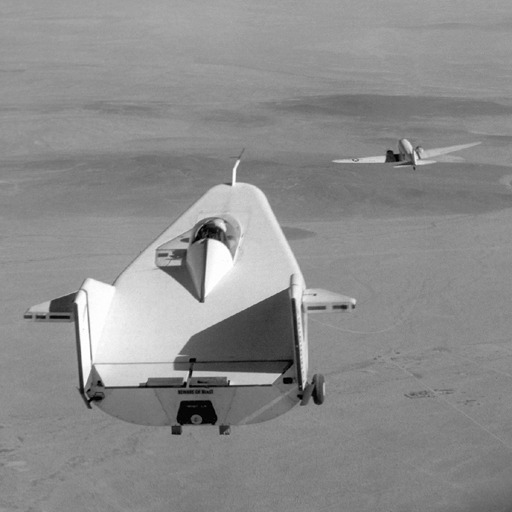
\includegraphics[width=8cm, height=8cm]{original_img.jpg}
\end{center}
\begin{center}
\begin{caption}
\caption{Input image}
\end{caption}
\end{center}
\end{graphics}\\
\noindent \textbf{Output image for 4-connectivity:}\\
\begin{graphics}
\begin{center}
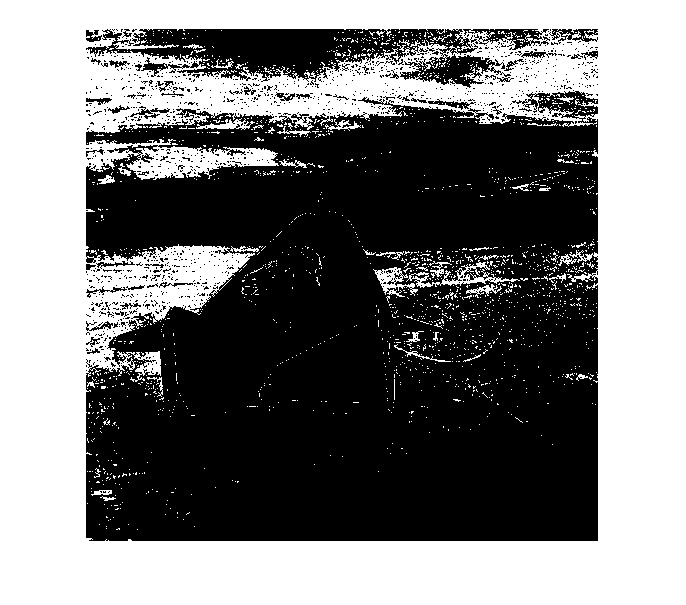
\includegraphics[width=11cm, height=11cm]{4-conn_img.jpg}\\
\end{center}
\end{graphics}
\clearpage
\noindent \textbf{Output image for 8-connectivity:}\\
\begin{graphics}
\begin{center}
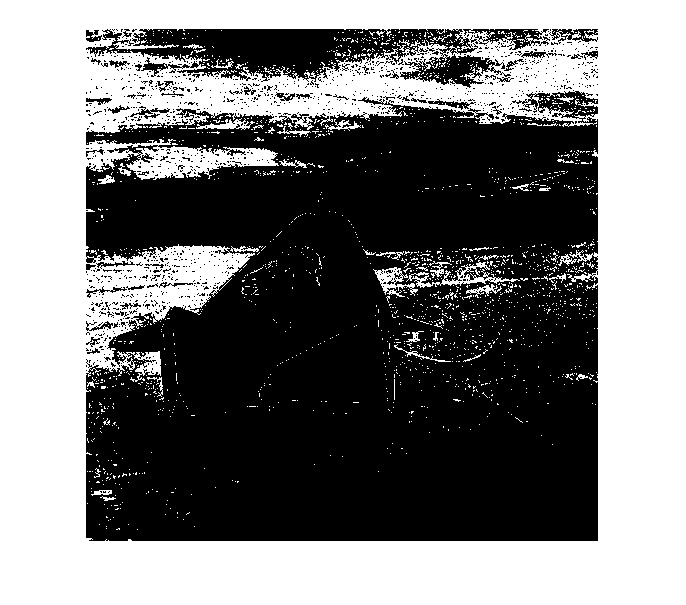
\includegraphics[width=11cm, height=11cm]{8-conn_img.jpg}
\end{center}
\end{graphics}

\newpage

\section{Solution for question No. 6}

\noindent The functions defined in the code are as follows:\\

\noindent \textbf{1. create\_rectangles():}\\
\noindent \textit{\textbf{Input arguments:-}} Size of the image (MXN), No.of the border pixel(bor), No. of the rectangles(n), starting pixel width of the rectangles(w1),ending pixel width of the rectangles(w2), Alpha(fixed ratio of hieght to width)(A),orientation of the rectangles(horizontal or vertical)(o1 and o2).\\
\noindent \textit{\textbf{Output arguments:-}} That gives the n rectangles with fixed ratio of height and width and orientation chosen as in the input by the user.\\

\noindent \textbf{2. member():}\\
\textit{\noindetnt{\textbf{Input arguments}}}- Any array(here b), Valued to be checked in the array(here a(row,col)). \\
\textit{\noindetnt{\textbf{Output arguments}}}- returns value of 'y' 1 if the value lies in array else 0.\\ 
 
\noindent \textbf{3. intensify():}\\
\noindent \textit{\textbf{Input arguments:-}} image in the form of matrix(I\_mat), thickness of border in terms of pixels(bor), size of the matrix(MXN).\\
\noindent \textit{\textbf{Output arguments:-}} displays and saves the final image.\\

\noindent \textbf{Explanation for the algorithm}:\\

\noindent This algorithm is coded using the basic inbuilt commands and only allowed inbuilt functions mentioned in the assignments. The functions that are used in that algorithms are manually defined with the help of basic commands. These functions saved as .m files in the same folder to execute. \\

\noindent \textbf{Step-1:} Drawing an image in the form of matrix of dimensions MXN which contains only white intensity  pixel value(1). The values of M\&N are the user define.\\ 

\noindent \textbf{Step-2:} To draw the border of width(bor), where `bor' is the no. of pixels present in the width of border, thickness of the border is user define.\\
\noindent In the above image, the peripheral pixels are assigned to the 0 value to obtain black colour border.\\

\noindent \textbf{Step-3:} Creating the n no. of rectangles, where n is user define.\\
\begin{itemize}
    \item Select the range of width from w1 to w2. Random points are those where one of the corner of rectangle lies. These values of width will start from w1 and next point will be the sum of w1 and step size. The step size is the difference between the w1 and w2 and divided by the no. of the rectangles.
    \item If the random point lies on the border then it will be discarded and loop will run to get another random point.
    \item If random point does not lies on border than it will be consider as valid point and added to the rand\_pos[ ] array.
    \item By the help of height to width ratio(alpha) rectangles are formed. These rectangles will be vertical, horizontal or both type on the basis of user defined orientation value. If the user gives any one input for orientation is 1 then rectangles are vertical and any one input for orientation is 2 then rectangles are vertical.
    \item if the rectangles are exceeding the image dimensions   then it will take next random point and generate rectangles, this will be repeated until the total rectangles less than or equal to the user input value.
    \item If user wants both type of rectangles then he/she should enter input orientation input values 1 and 2. It will start with vertical rectangles after that horizontal and repeat the same process as mentioned above.
    \item If the no. of rectangles formed in the image are less than the requirement as per user define then the dimensions of the image will be double. The random points are also change to form new rectangles of same alpha.
    
\end{itemize}

\noindent{\textbf{Step-4:}} Displaying final image considering different foreground and background pixels.

\begin{itemize}
    \item For displaying the final image the user input will be taken, if the user wants the simple black and white image then it will simply display the gray scale image and save tool is activated.
    \item If the user wants to add the intensities then foreground and background pixel intensities are taken as input in a range, with the step size and these intensities are distributed in foreground and background uniformly.\\
\end{itemize}

\noindent \textbf{TEST CASE:}\\
\noindent \textbf{Inputs for the code:}\\
\noindent M=250\\
N=250\\
bor=3\\
n=7\\
w1=50\\
w2=200\\
Alpha(A)=3\\
o1=1\\
o2=2\\
\\
\noindent \textbf{Output image without intensities:}\\
\begin{center}
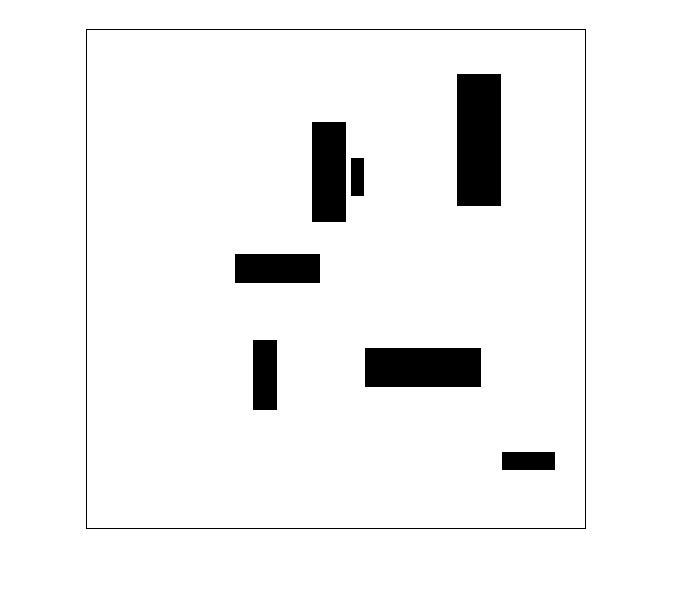
\includegraphics[width=8cm, height=8cm]{without_intensities.jpg}
\end{center}

\newpage
\noindent \textbf{Input for the code:}\\
\noindent M=250\\
N=250\\
bor=3\\
n=7\\
w1=50\\
w2=200\\
Alpha(A)=3\\
o1=1\\
o2=2\\
Start value of Vf=20\\
step value=2\\
End value for Vf=100\\
Start value for Vb=200\\
step value=2\\
End value for Vb=250\\
\\
\noindent \textbf{Output image with intensities range provided:}\\
\begin{graphics}
\begin{center}
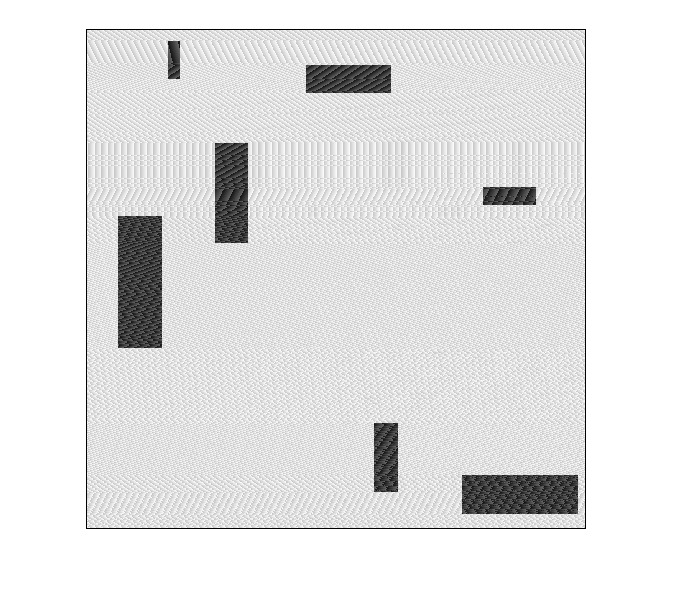
\includegraphics[width=8cm, height=8cm]{with_intensities.jpg}
\end{center}
\end{graphics}


 
\newpage

\noindent \section{Solution for question no.7}\\

\noindent Here as per discussed in the assignment, the real life application of long range iris detection will be discussed from the point of Autonomous machine vision in robotics.\\

\noindent \textbf{The idea:}\\
\noindent Robotics has evolved excellently in these decades. And more of the emphasis is made on the implementation of the advanced AI techniques. Our idea or application we want to roughly float here is to implement long range iris detection in the robotic visual sensors to recognize its owner from quite a distance and reserve its services only for its owner.
Such applications can be used for personal assistance, or for some personally customized tasks. As per mentioned, this article will not cover the technicalities for the implementation, but will give the idea about the use of Digital Image Processing techniques to develop such complex algorithm.\\
\noindent \textbf{•	Why iris?}\\ 
\noindent Biometric identification has penetrated into too many helpline and identity for citizenship in most of the nations across the world in UK, USA, Canada, Argentina etc. India started the scheme of Adhaar cards since 2016. Biometric recognition consists of bifurcating one subject from other by taking an unique signature specimen from their body, data obtained from the specimen of one particular subject must be different from the specimen obtained from other subject. 

Such recognition schemes involve facial recognition, fingerprint detection, Gait recognition, Iris recognition etc. This article will focus more on Iris recognition. Iris is a complicated texture inside the stroma of an eye which resizes the pupil to control light entering the eye. This texture is very complicated, unique for each individual, don’t have much impact of aging  and has very less genetic penetration, has more degree of freedom than face and fingerprint detection methods, which are the major advantages of using this trend. \\


\noindent \textbf{•	How can it be done?}\\
\noindent The step by step process would be to acquire an image through visual sensors and to analyze whether the data of texture of the iris of the owner can be extracted from the image with sufficient image filtering algorithms or not. If required we can simply implement Histogram matching or contrast enhancement techniques.\\

\noindent Step by step process to extract the image would be.\\ 

\noindent \textbf{Segmentation of the iris contour in the image:-}\\
\noinedt Segmentation is simply differentiating the main data with respect to their co-ordinates in the space. Unique texture of the iris in between the inner and outer boundary of the iris and its circular edge can be found by the maximum response in the pre-defined boundary. As we are taking about the circular structure we can simply convert (x,y) co-ordinates into polar co-ordinates i.e (r,Th) keeping the center of pupil as origin.\\
\noindent Most of the times it is not possible to get the complete circle with the upper and lower eyelids covering the pupil, thus we get more of a arc rather than circular contour.\\

\noindent \textbf{Normalization of the image:-}\\
Normalization is to bring the data scaled differently in different specimens to same pre-defined scale, for the sake of simplicity of calculations and processing the data for further algorithm. This is necessary because the pupil dilution will be different from individual to individual. And thus the contour for the iris may vary and scaled differently, Thus to compare it with the existing database normalization is must.\\
And the added advantage through normalization is inclination of head of the personnel won’t matter as the normalization will be in terms of (r, Th) and it will be simple translation operator.\\

\noindent \textbf{Encoding:-}\\
Encoding is to take out the most discriminative, but compact data from the normalized image and assign it the complex valued bit. Phase information matters the most as amplitude values can be simply affected by the surrounding environment like external light. Once these phase bits are acquired they are used for matching the image with the date based image and similarity between both of them is measured. Such an array of contains approximately 2048 phase bits and is called Iriscodes.\\

\noindent \textbf{Matching of the images:-}\\
This is the important and final part where the recognition really occurs. Here the Iriscode from the normalized image and the Iriscode of the data based image are compared and the similarity score is computed.\\

\noindent \textbf{Long range iris recognition:-}\\
\noindent The step by step procedure explained above is common algorithmic approach for iris recognition. But, for the long range iris detection, the major contribution had done from the hardware implementation.\\
In beginning lot many approaches were made to detect the iris from the long range by implementing various image sensors, where the constraints that hurdled mainly are.\\
\begin{itemize}
    \item Subject should be positioned in between 0.5m – 1m distance and should stay still.
    \item It was impossible to get optimized frame rate to get accurate image of iris, when subject is moving.
    \item It was impossible to get optimized frame rate to get accurate image of iris, when subject is moving.
    \item  Even getting the optimized capture volume for algorithm to run successfully was quite a challenge.
\end{itemize}
\noindent Major revolution came with the introduction on an “Eagle Eye” system by Bashir et al. this technique uses three cameras. 1) Fixed scene camera for multiple face tracking, 2) Face camera for face detection, 3) NIR iris cameras for iris detection. These cameras are setup on Pan-Tilt Unit, in such a way that when face camera detects a face, the iris on that face is aligned along with the iris camera (Here the Fixed scene camera has more field of view, but less resolution. But, iris camera has high resolution but less field of view). \\

Such use of multiple cameras is then advanced with implementing the cameras with different resolutions and better algorithms for face recognition and then focusing on iris. By year 2011, Cylab presented an iris imaging system capable of getting the high resolution images from the stationery as well as moving subject at a distance of 8 – 12m. For moving subjects the additional camera was put to take velocity into consideration.\\
\begin{figure}
\begin{center}
    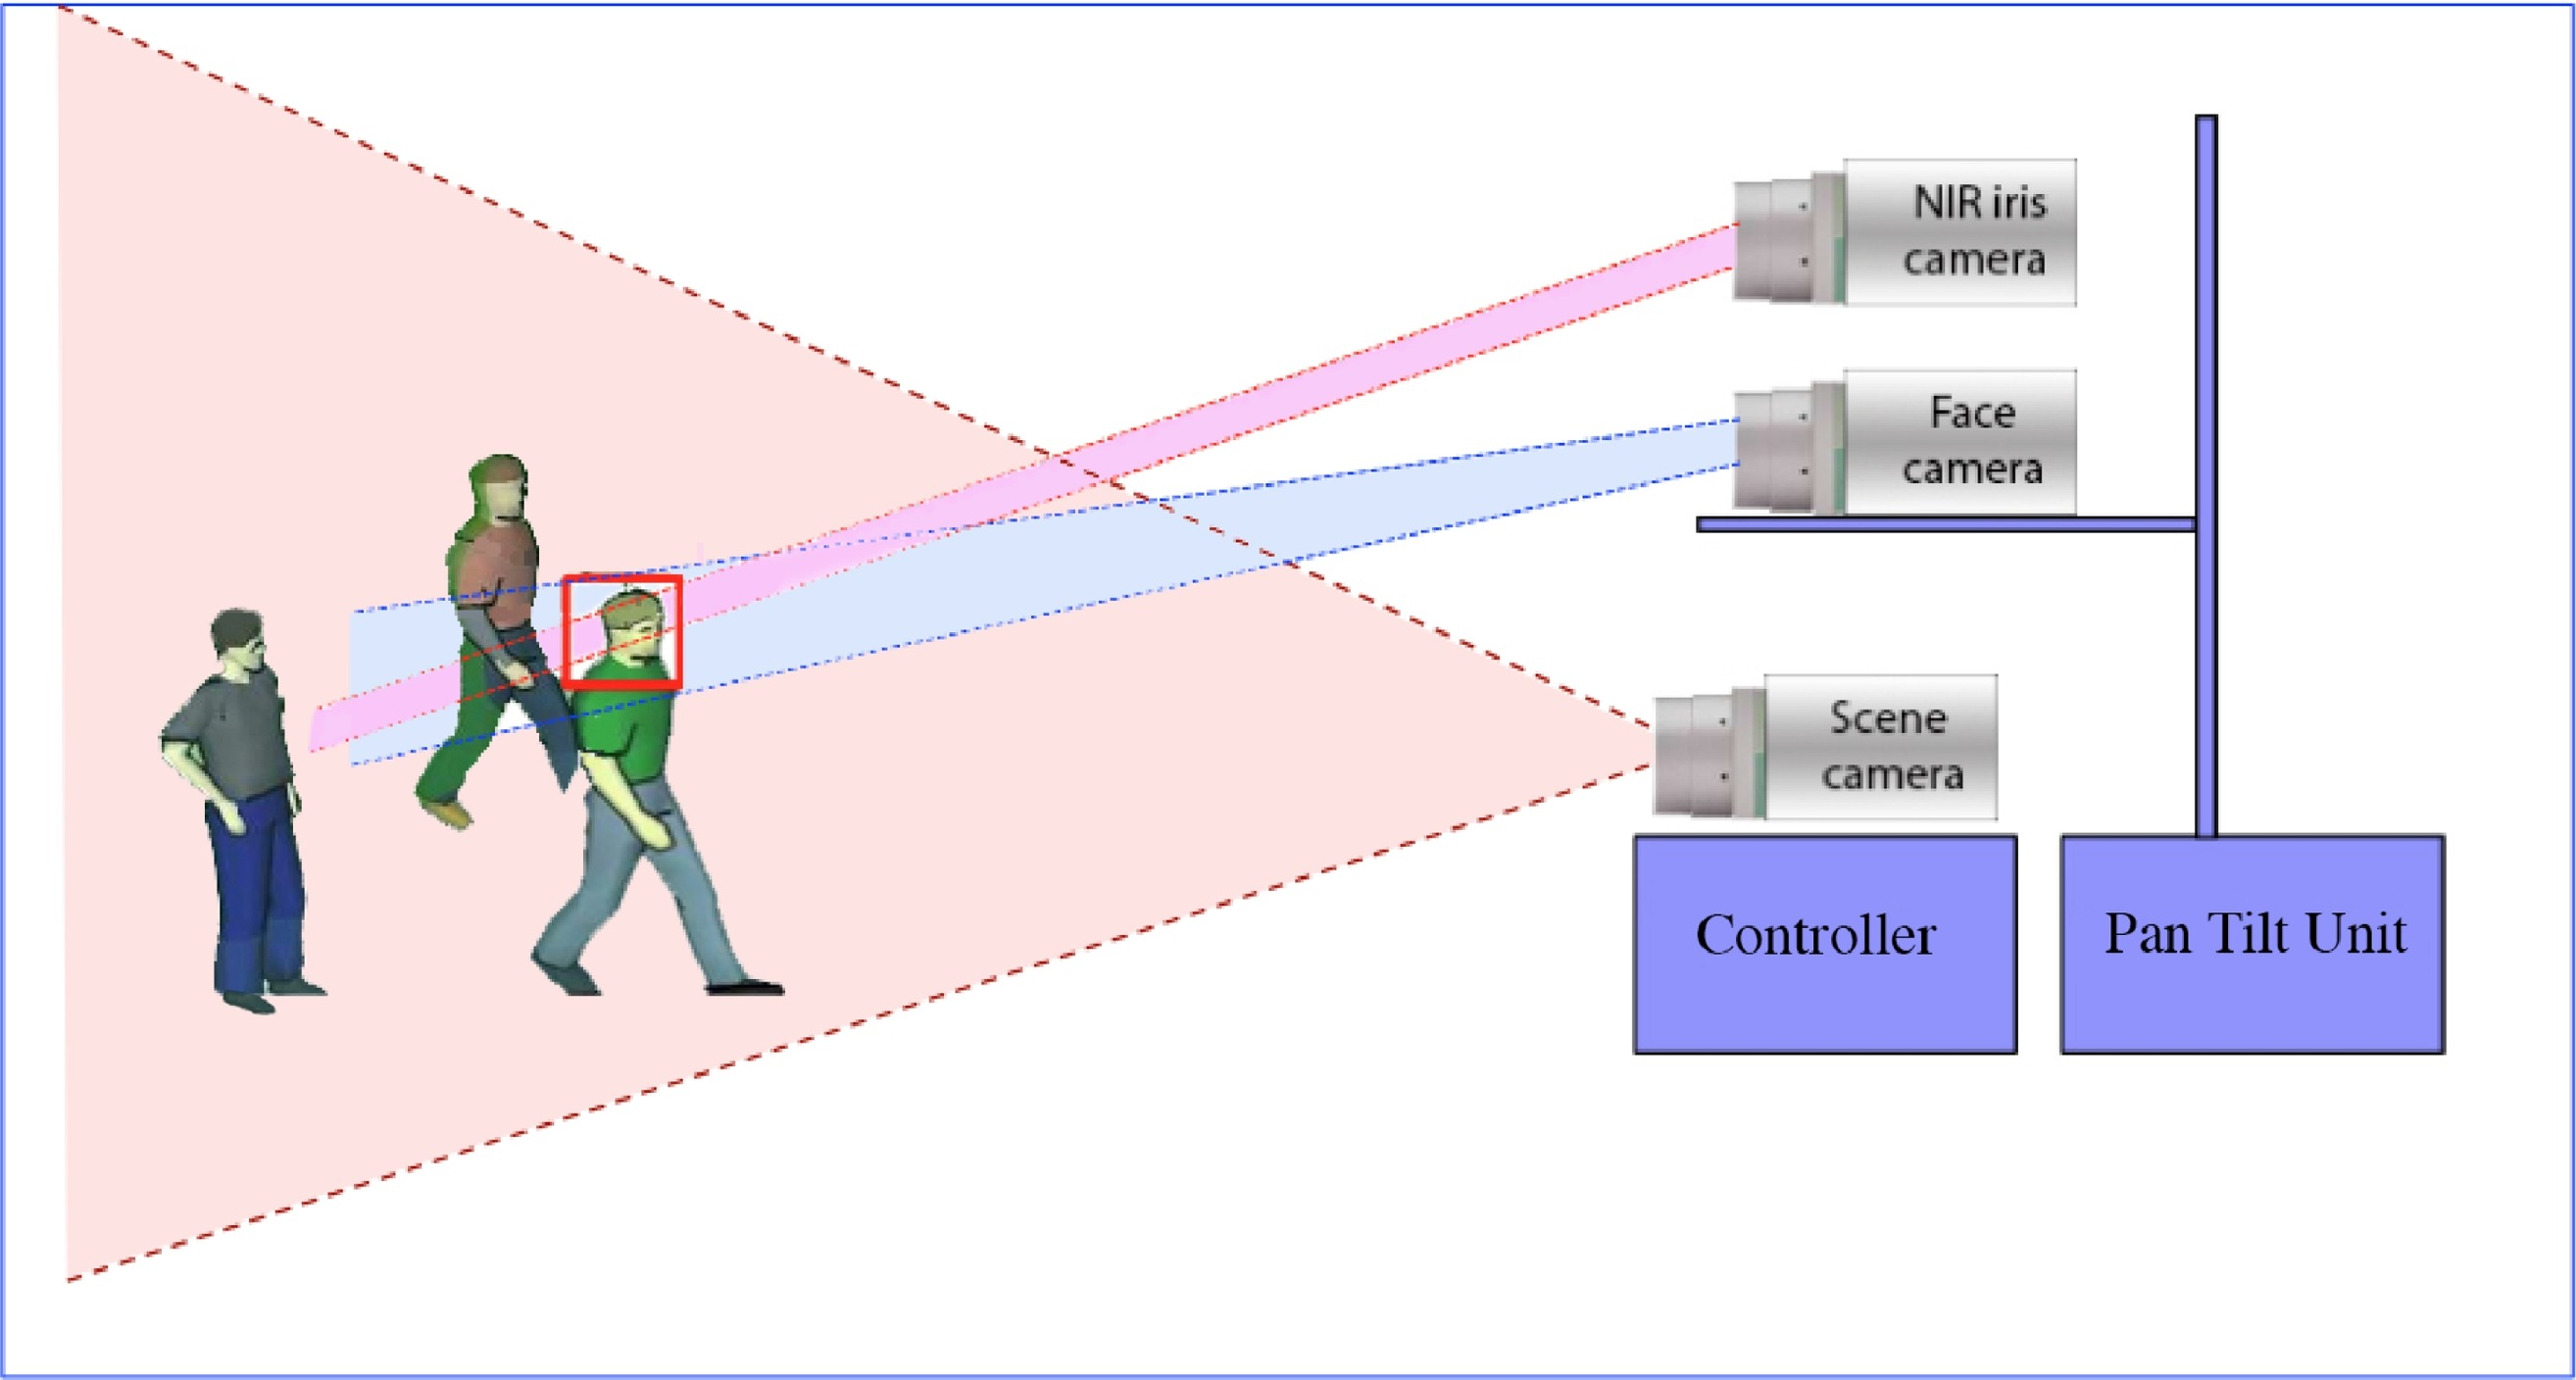
\includegraphics[width=14cm, height=9cm]{men.jpg}
    \caption{Typical presentation of three cameras working.}
\end{center}
\end{figure}

\noindent There has been so much advancement in hardware implementation of the sensors. But as we are dealing with the contribution of Digital signal processing, much of its contribution lies in the software implementation.\\

\noindent \textbf{Quality of image:-}\\
\noindent Image quality is taken into consideration, because the images taken from a distance may lack the consistency. According the frame rate of the cameras, this step can help us to get the image which can provide the complete information and to discard the poor quality images.\\

\begin{figure}
\centering
    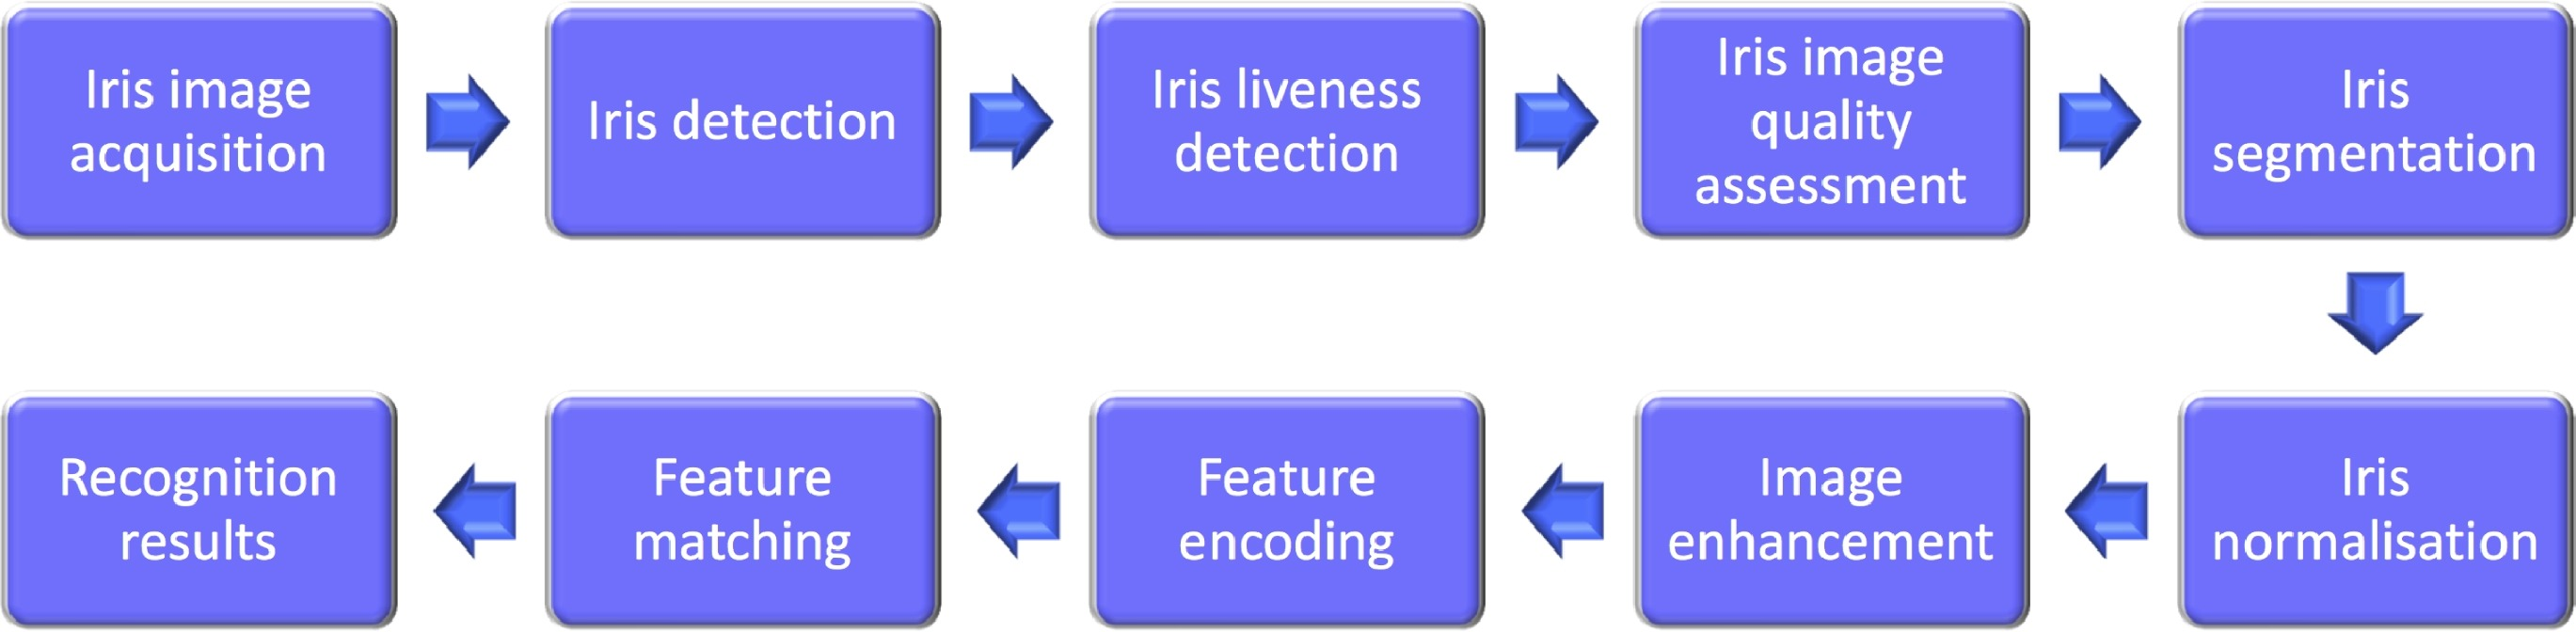
\includegraphics[width=14cm, height=5cm]{blockdia.jpg}
    \caption{Algorithm to be adopted for long range iris recognition}
\end{figure}\\

\noindent \textbf{Spoof detection:}\\

\noindent Here spoof detection mainly means to check the liveliness of the iris, i.e the system shouldn’t be fooled by a fake iris structure or an printed iris image on the paper. To do so, the hardware implementation of the sensors taking consideration of the veins in the eye and reporting back can work.\\
\npindent Or the algorithm which can detect the liveliness of the eye using
\begin{itemize}
    \item 	Pupil size oscillations.
    \item Periodic eye blinking.
    \item Iris muscle deformation under varying illumination
    \item Local bit pattern
\end{itemize}
\noindent can also help in spoof detection.\\

\noindent \textbf{Iris segmentation:}\\
\noindent Iris segmentation is quite difficult as the image is acquired from long range. The circular boundary assumption may not work due to occlusions, varying intensity, surrounding environment and noise, etc. To eradicate them using various machine learning techniques to bifurcate between iris pixels \& no-iris pixels.

\noindent Thus, these procedures can be implemented using filtering techniques in Digital Signal Processing. And using such hardware implementations, we can upgrade the visual sensors in robots and can achieve the individual iris recognition for the distance.\\

\noindent \textbf{References:}\\
\item	Nguyen, K., Fookes, C., Jillela, R., Sridharan, S. and Ross, A., 2017. Long range iris recognition: A survey. Pattern Recognition, 72, pp.123-143.
\end{document}
\end{document}